Embarking on the findings of this chapter, we transition from the established COMSOL modeling workflow to the critical stage of validating theoretical concepts through the lens of computational analysis. The essence of this chapter is twofold: first, to harness the computational prowess of COMSOL in substantiating key optical phenomena such as anti-reflectivity thus corroborate our simulation outcomes with theoretical models; and second, to attempt to model the simplest Passive Daytime Radiative Cooling devices (PDRCs) at Hudgings Lab by showing how their reflectance varies with wavelength.

Our investigation begins with an empirical analysis of anti-reflective behaviors, examining both simple and composite multilayer arrangements. These simulations are meticulously compared to the theoretical predictions presented in \emph{Introduction to Optics} by Frank L. Pedrotti et al., ensuring our findings adhere to the rigorous standards of optical precision.

We delve into the intricacies of high reflectance by simulating stacks of alternating high and low refractive index layers, shedding light on the nuanced ways layer configurations impact reflectance. These insights are bench-marked against scholarly literature, reinforcing the accuracy of our models.

Aligning with practical applications, we employ the Fresnel equations to map out the reflection coefficient, for both the transverse electric (TE) and transverse magnetic (TM) polarization, against the angle of incidence. The insights gleaned here will serve to consolidate our understanding of various optical phenomena.

Moreover, the thesis explores the layered design of PDRCs. By systematically layering glass, silver, and Polydimethylsiloxane (PDMS), we dissect the optical properties crucial to the development of passive cooling systems.

This chapter stands at the intersection of physics and simulation, merging the realms of theory and experimentation. The collection of results and graphs here encapsulate more than just data; they are catalysts for continuous inquiry and deeper understanding of optical physics as it related to PDRCs.

\section{COMSOL: Modeling Anti-reflectivity.}
Recalling the formula for the reflectance of a two-layer anti-reflecting film, given by equation \ref{reflectance for 2-layer antireflecting films}, and assuming light strikes normally, we have:

\begin{equation}\label{reflectance for 2-layer antireflecting films - chap4}
    R = \left(\frac{n_0n_2^2 - n_sn_1^2}{n_0n_2^2 + n_sn_1^2}\right)^2
\end{equation}

Here, we anticipate zero reflectance when the expression in the numerator becomes zero, leading us to equation \ref{zero reflectance criterion}, which stipulates the condition for achieving no reflectance:

\begin{equation}\label{zero reflectance criterion - chap4}
    \frac{n_2}{n_1} = \sqrt{\frac{n_s}{n_0}}
\end{equation}

This relationship delineates the necessary ratio between the refractive indices of the layers that leads to a reflectance of zero.

When working with a glass substrate of refractive index $n_s = 1.5$ and air of refractive index $n_0 = 1$, the ideal refractive index ratio, $\frac{n_2}{n_1}$, is calculated to be $\sqrt{1.5} \approx 1.225$.

In COMSOL, our goal is to identify and define (in our parameters table) two materials for the double-layer structure that closely match this ratio to maximize anti-reflective properties. It's crucial to note that within the visible spectrum, ranging from 400 to 700 nm, each wavelength uniquely interacts with materials based on their specific refractive index at that wavelength. This variability, known as dispersion, means that optimal thickness and refractive indices for minimizing reflectance at one wavelength may not be as effective at another. While it's challenging to select materials that precisely align their refractive indices to achieve exactly zero reflectance, our aim is to get as close to 0\% reflectance as practically possible.

The limitation of a quarter-wavelength layer is its selective reflectivity; it effectively eliminates reflection at a specific wavelength but substantially reflects at other wavelengths in proximity. Additionally, its performance varies significantly with the angle at which light strikes the surface. A viable solution to overcome this is the application of multilayer coatings. These coatings, compared to their single-layer counterparts, tend to lower the reflection coefficient over a broader spectrum and accommodate a greater diversity of tangible materials \cite{pedrotti_introduction_2007}.

In the following section, we will compare the reflectivity of two distinct multilayer coatings across an extensive spectral range. The analysis will cover a dual-layer, quarter-quarter wavelength coating, and a triple-layer, quarter-half-quarter wavelength coating. It will be demonstrated that the triple-layer coating achieves a more uniform low reflectance throughout the majority of the visible light spectrum.


% TODO: CHANGE the title of this subsection

\subsection{Anti-reflectance Layers: Setup}

The pursuit of anti-reflective coatings leads us to the utilization of thin film dielectrics within COMSOL. In line with the criteria for zero reflectance, the first dielectric film, starting from the base, is cerium trifluoride (CeF3) with a refractive index of 1.63, while the second film is magnesium fluoride (MgF2) with a refractive index of 1.38. The refractive index ratio of approximately 1.181 aligns closely with the optimal ratio of 1.225. As established in chapter 2, effective anti-reflectivity for a dual-layer arrangement requires each film to be a quarter-wavelength in thickness, which corresponds to the wavelength at which minimal reflectance is desired.

In our enhanced three-layer structure, designed to broaden anti-reflectivity across a larger wavelength spectrum, the middle layer is a half-wavelength film of zirconium dioxide (ZrO2), chosen for its refractive index of 2.1. This multi-layer configuration allows for increased anti-reflective performance compared to the more wavelength-specific two-layer model.

This screenshot from the COMSOL desktop highlights the configuration for modeling anti-reflective coatings. Pay particular attention to the 'Film Properties' area within the 'Thin Dielectric Film' settings where the quarter-wavelength calculation is outlined.

\begin{figure}[ht!]
  \centering
  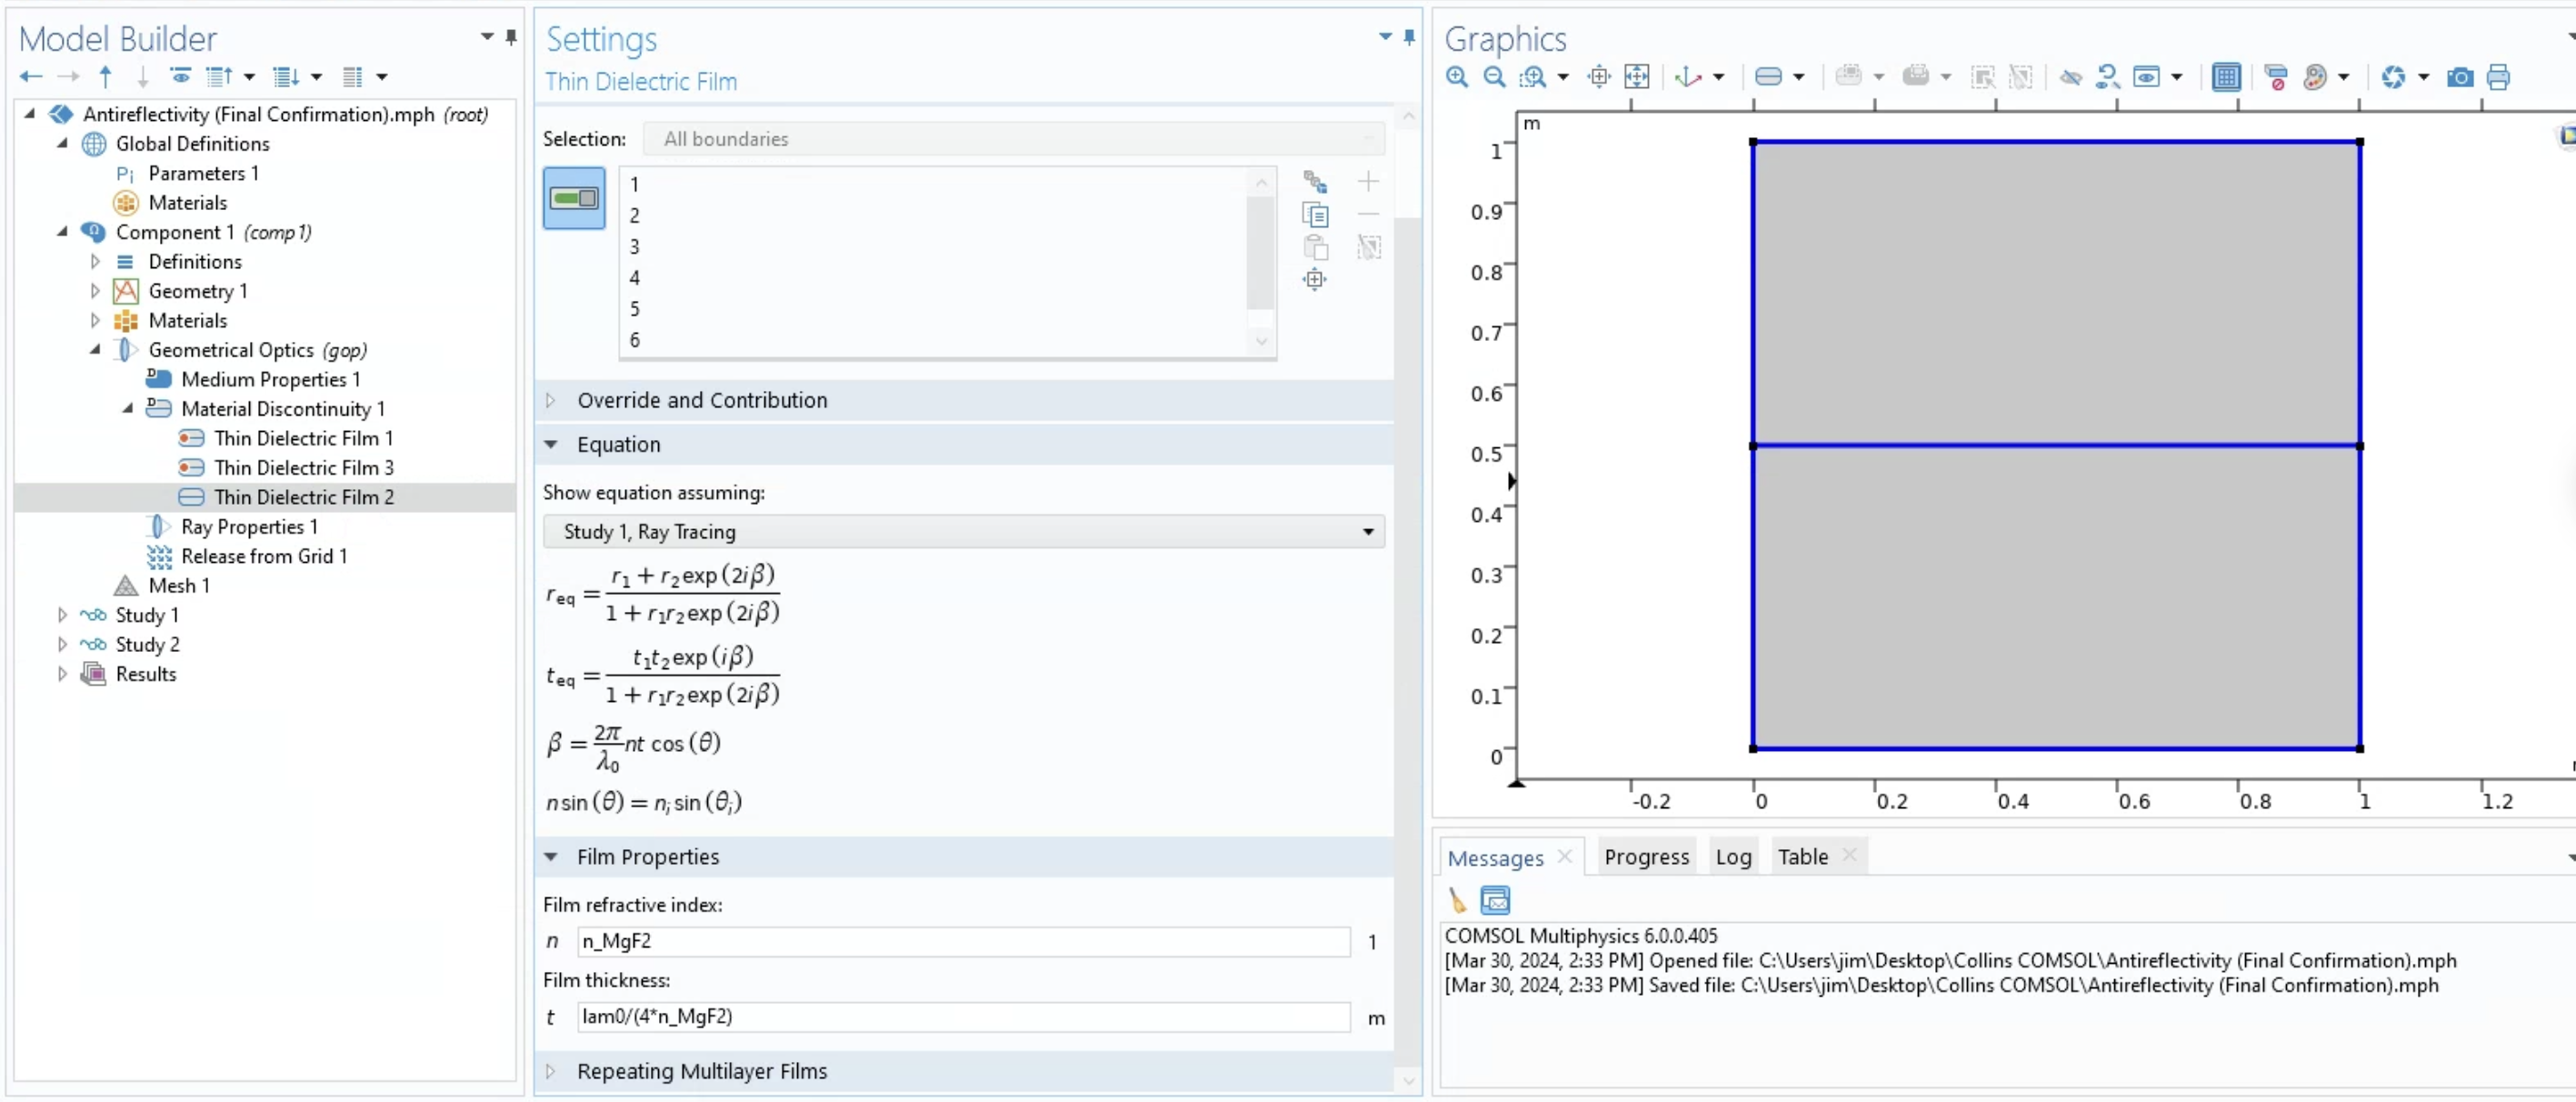
\includegraphics[width=0.4\textwidth]{Chapters/Figures/Chapter 4 Figures/COMSOL Desktop Showcasing Antireflectivity Setup.png}
  \caption{COMSOL desktop setup showcasing anti-reflectivity modeling.}
  \label{fig:COMSOL desktop showcasing antireflectivity}
\end{figure}

Here, the findings from the anti-reflectivity modeling using CeF3 and MgF2 for the quarter-quarter wavelength combination, as well as CeF3, MgF2, and ZrO2 for the quarter-half-quarter wavelength setup, are presented.

\begin{figure}[ht!]
  \centering
  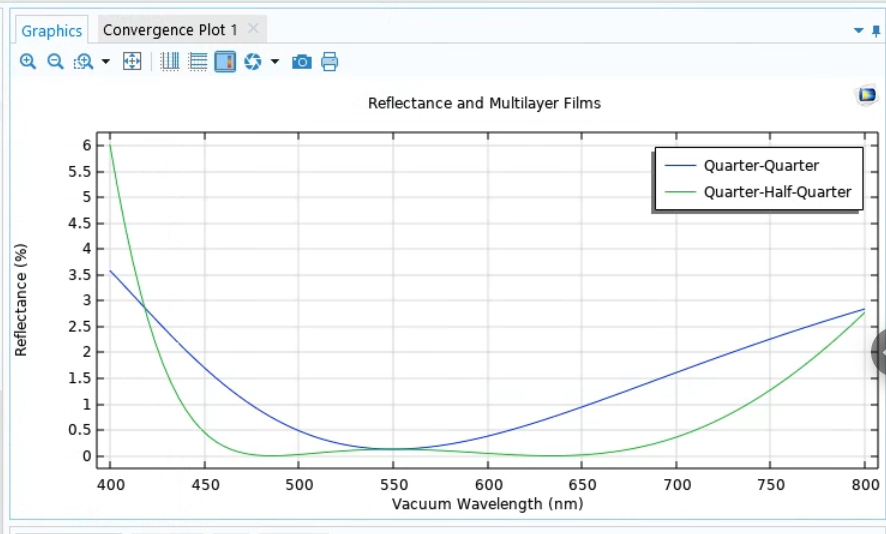
\includegraphics[width=0.4\textwidth]{Chapters/Figures/Chapter 4 Figures/Quarter-Half-Quarter.png}
  \caption{Illustration of the reflectance behavior for two anti-reflective coating configurations across the visible light spectrum. The blue line indicates the performance of a quarter-quarter wavelength coating, whereas the green line shows the effect of a quarter-half-quarter wavelength coating.}
  \label{fig:both quarter-quarter and quarter-half-quarter}
\end{figure}

In the quarter-quarter wavelength design, we employ two layers, each precisely a quarter of the desired wavelength in thickness. While the aim is to achieve minimal reflectance at a particular wavelength, the actual reflectance seldom reaches absolute zero due to the inherent limitations of material characteristics.

On the other hand, the quarter-half-quarter arrangement introduces an additional layer, half a wavelength thick, nestled between two quarter-wavelength films. This configuration is tailored to minimize reflectance across an extended spectrum of wavelengths.

Such multi-layered coatings surpass the effectiveness of single-layer films for anti-reflective purposes by accommodating a wider wavelength range. This versatility is particularly beneficial in applications where reducing reflection is paramount, such as in the manufacturing of optical lenses.

\subsection{Verification of Theoretical Results from Optics Literature}

This section aims to validate the principles outlined in \emph{Introduction to Optics} by Frank L. Pedrotti et al. through the simulation of multilayer film behavior, ensuring our computational results align with established optical theories.

Beginning with a straightforward approach, we examine the reflectance across various wavelengths for three distinct multilayer film configurations:
\begin{enumerate}
    \item Films with quarter-quarter wavelength thickness.
    \item Films with quarter-half wavelength thickness.
    \item Films with quarter-half wavelength thickness, incorporating a different material for the half-wavelength layer.
\end{enumerate}

\begin{figure}[ht!]
  \centering
  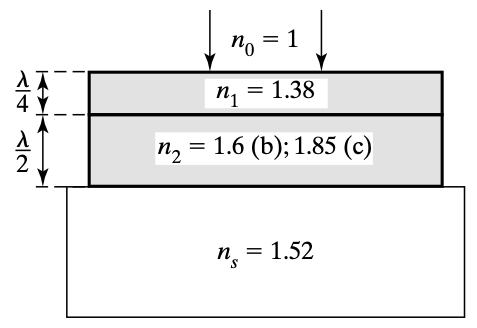
\includegraphics[width=0.4\textwidth]{Chapters/Figures/Chapter 4 Figures/Antireflecting Double Layer using Quarter and Half-Wavelength Thickness Films Layout.png}
  \caption{Antireflective double-layer arrangement. Source: \cite{pedrotti_introduction_2007}}
  \label{fig:antireflective_double_layer}
\end{figure}

We first examine films with quarter-quarter wavelength thickness. The reference from Pedrotti et al. specifies the lower thin dielectric layer as $\text{ZrO}_2$ and places $\text{CeF}_3$ directly above. The choice of materials is flexible, provided they adhere to the optimal ratio criterion for antireflectivity as defined in equation \ref{zero reflectance criterion - chap4}. This results in a refractive index ratio of $\frac{n_2}{n_1} = \frac{2.1}{1.65} \approx 1.273$, aligning closely with the ideal ratio of approximately 1.225 for normal incidence, given a substrate refractive index ($n_s$) of 1.5.

Expanding the spectrum of low reflectance within the visible region becomes achievable by diverging from the constraint of equal quarter-wavelength ($\lambda/4$) coatings. By integrating a layer of quarter-wavelength thickness as the second layer (considered from the bottom upwards), we attain more extensive zones of diminished reflectance. Consequently, in the scenario of item 2, we employ magnesium fluoride ($\text{MgF}_2$), characterized by a refractive index of 1.38, as the quarter-wavelength thick material. The intermediate half-wavelength layer utilizes aluminum oxide, with a refractive index of 1.60. For item 3, thorium dioxide, featuring a refractive index of 1.85, serves as the material for the half-wavelength thick layer, as noted in \cite{pedrotti_introduction_2007}.

For the specific wavelength of 550 nm, where the thicknesses of the quarter-wavelength ($\lambda/4$) and half-wavelength ($\lambda/2$) layers are calculated, the half-wavelength layer does not influence reflectance. In this case, the double-layer system acts akin to a solitary quarter-wavelength layer, resulting in a reflectance of 1.3\%. At wavelengths close to 550 nm, the presence of the half-wavelength layer contributes to maintaining reflectance levels below those achieved by a two quarter-wavelength layers. Below is the plot illustrating reflectance against wavelength for scenarios 1 through 3:

The graph below illustrates anti-reflectivity trends as detailed in the Optics textbook, indicating that while the reflectance at a wavelength of 550 nm stands at approximately 1.3\%, this value surpasses the performance of the quarter-quarter wavelength coating. Nevertheless, reflectance stays below this threshold across a wide wavelength span, extending from roughly 420 to 800 nm. This suggests that alternative configurations for dual-layer reflective films could be viable if the layers are not strictly constrained to quarter-wavelength multiples.

\begin{figure}[ht!]
  \centering
  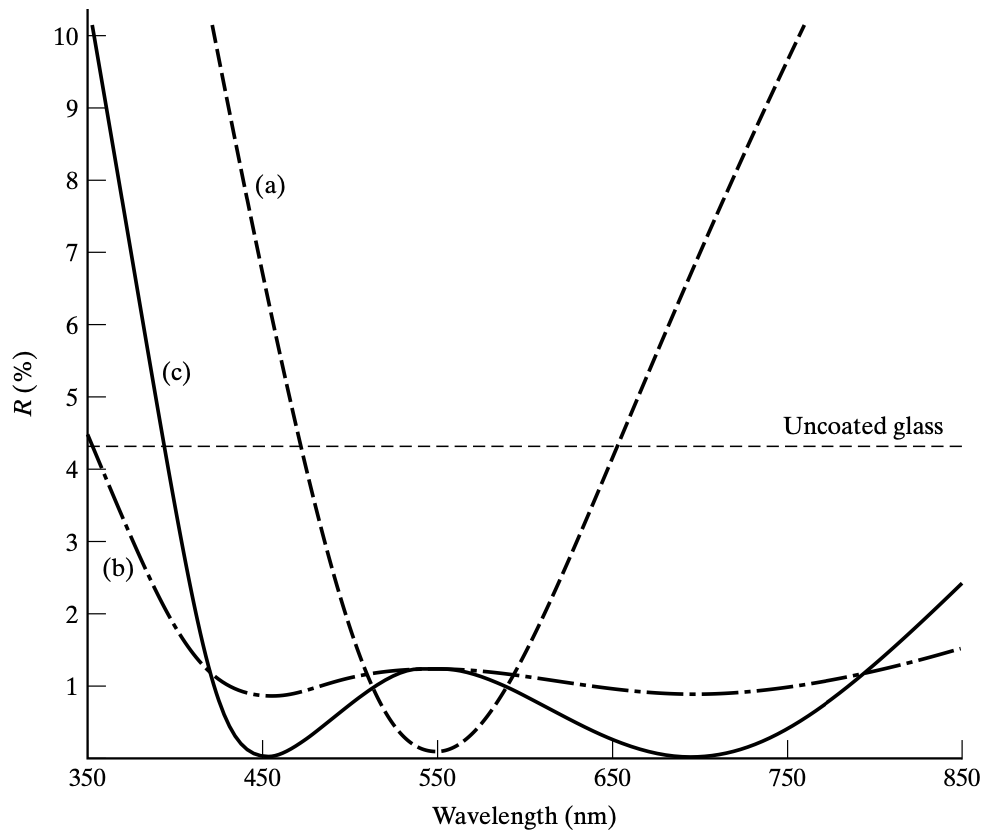
\includegraphics[width=0.4\textwidth]{Chapters/Figures/Chapter 4 Figures/Antireflectivity Graphs in the Optics Book.png}
  \caption{Anti-reflectivity Graphs as shown in the Optics Textbook. Source: \cite{pedrotti_introduction_2007}}
  \label{fig:antireflectivity graphs in the Optics book}
\end{figure}

Presented below are the modeled results for scenarios (a), (b), and (c) as detailed previously, with corresponding legends found in figure \ref{fig:antireflectivity graphs in the Optics book}. Notice how each individual plot resembles each plot in figure \ref{fig:antireflectivity graphs in the Optics book}.

\begin{figure}[ht!]
  \centering
  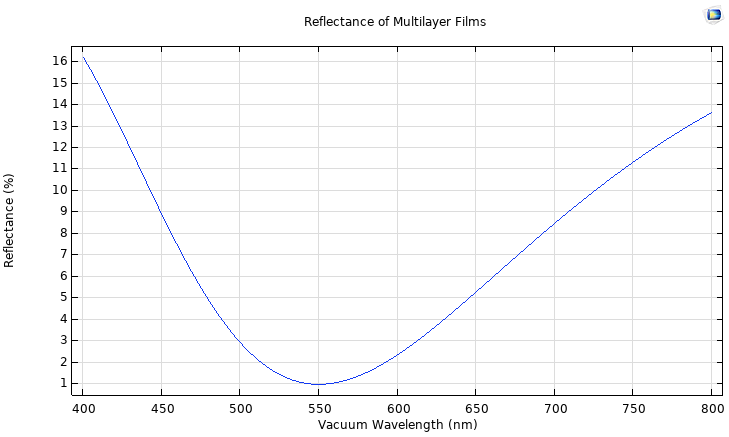
\includegraphics[width=0.4\textwidth]{Chapters/Figures/Chapter 4 Figures/Antireflective Figure a.png}
  \caption{Modeling results of an anti-reflective coating with two layers, each a quarter-wavelength thick.}
  \label{fig:Antireflective Figure a}
\end{figure}

\begin{figure}[ht!]
  \centering
  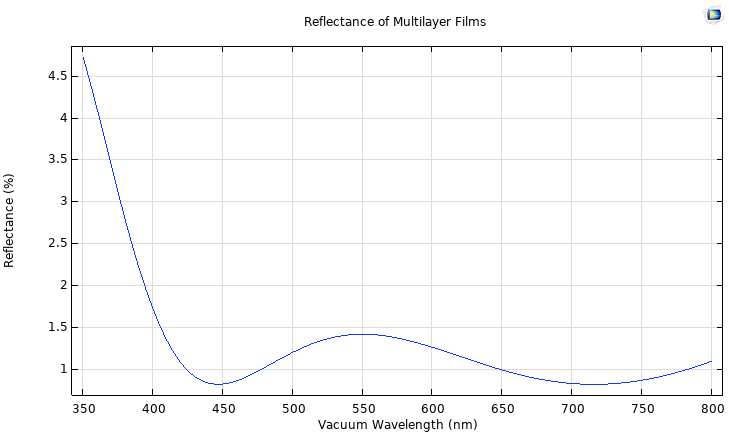
\includegraphics[width=0.4\textwidth]{Chapters/Figures/Chapter 4 Figures/Antireflective Figure b.png}
  \caption{Reflectance outcomes for an anti-reflective coating with a bottom layer a quarter-wavelength thick and a top layer half-wavelength thick, using a material with a refractive index of 1.6.}
  \label{fig:Antireflective Figure b}
\end{figure}

\begin{figure}[ht!]
  \centering
  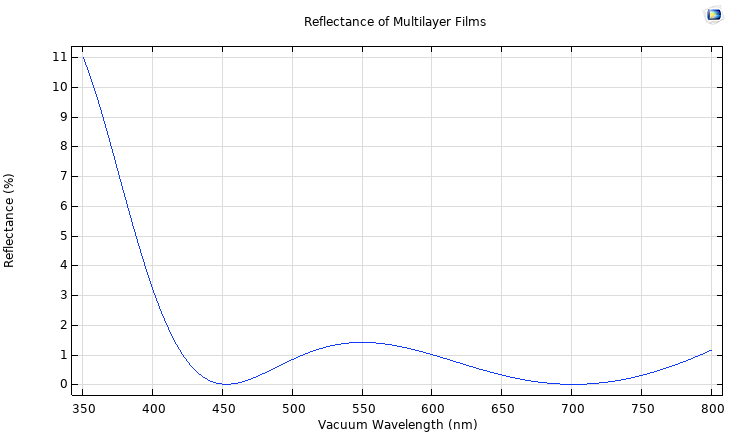
\includegraphics[width=0.4\textwidth]{Chapters/Figures/Chapter 4 Figures/Antireflective Figure c.png}
  \caption{Reflectance results for an anti-reflective double layer with a bottom layer a quarter-wavelength thick and a top layer half-wavelength thick, using a material with a refractive index of 1.85.}
  \label{fig:Antireflective Figure c}
\end{figure}

These results derive from the principles outlined in Chapter 2. Initially, the overall transfer matrix elements are calculated by multiplying the transfer matrices of the individual layers together. Within these calculations, the phase difference, $\delta$, varies with $\lambda$, aligning the film thickness with either $\lambda/4$ or $\lambda/2$ at the reference wavelength of 550 nm.

Subsequently, the reflection coefficient, as outlined in \ref{reflection coefficient in terms of transfer matrix terms}, is squared to produce reflectance as a wavelength function. COMSOL's Ray Optics module significantly simplifies this process by automating several steps, although careful consideration is needed for layer treatment, particularly regarding their classification as thin dielectric films.

\section{COMSOL: Modeling High Reflectance.}
To achieve anti-reflective properties, layers are arranged starting from the air and progressing through low-index to high-index materials before reaching the substrate. In contrast, for enhanced reflectivity, the sequence is reversed, starting from the air to high-index and then to low-index materials before ending at the substrate. This arrangement encourages multiple reflections of the incident light within the layered structure.

A combination of layers arranged to maximize reflectivity is known as a \emph{dielectric mirror}, \emph{high-reflectance stack}, or \emph{distributed Bragg reflector}. It's important to note that achieving high reflectance across the solar spectrum is a key factor for effective passive daytime radiative cooling, as previously discussed.

\begin{figure}[ht!]
  \centering
  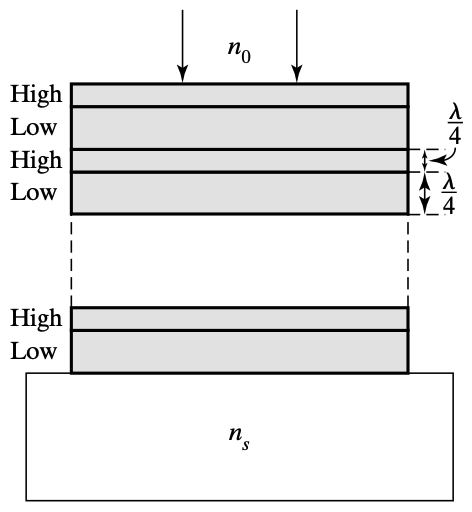
\includegraphics[width=0.4\textwidth]{Chapters/Figures/Chapter 4 Figures/High-Reflectance Stack of Double Layers.png}
  \caption{High-reflectance stack comprising double layers with alternating high and low refractive indices. Source: \cite{pedrotti_introduction_2007}}
  \label{fig:visualizing high-reflectance stack with alternating indices}
\end{figure}

\subsection{Verification of Theoretical Results from Optics Literature.}
The formula to ascertain high reflectance, $R$, at a chosen design wavelength ($\lambda_0$) for a specific layer arrangement is denoted by \ref{maximum reflectance equation}.

\begin{equation}\label{formula for optimal reflectance - chap4}
    R = \left[ \frac{ \left( \frac{n_0}{n_s} \right) \left( \frac{n_L}{n_H} \right)^{2N}  - 1 }{  \left( \frac{n_0}{n_s} \right) \left( \frac{n_L}{n_H} \right)^{2N}  + 1}  \right]^2
\end{equation}

Achieving maximal reflectance (100\%) occurs under the following conditions:
\begin{enumerate}
    \item As $N$, representing the count of layer pairs, becomes very large.
    \item When the ratio $\frac{n_L}{n_H}$ approaches zero.
\end{enumerate}

The optics textbook illustrates high reflectance with the following depiction:

\begin{figure}[ht!]
\centering
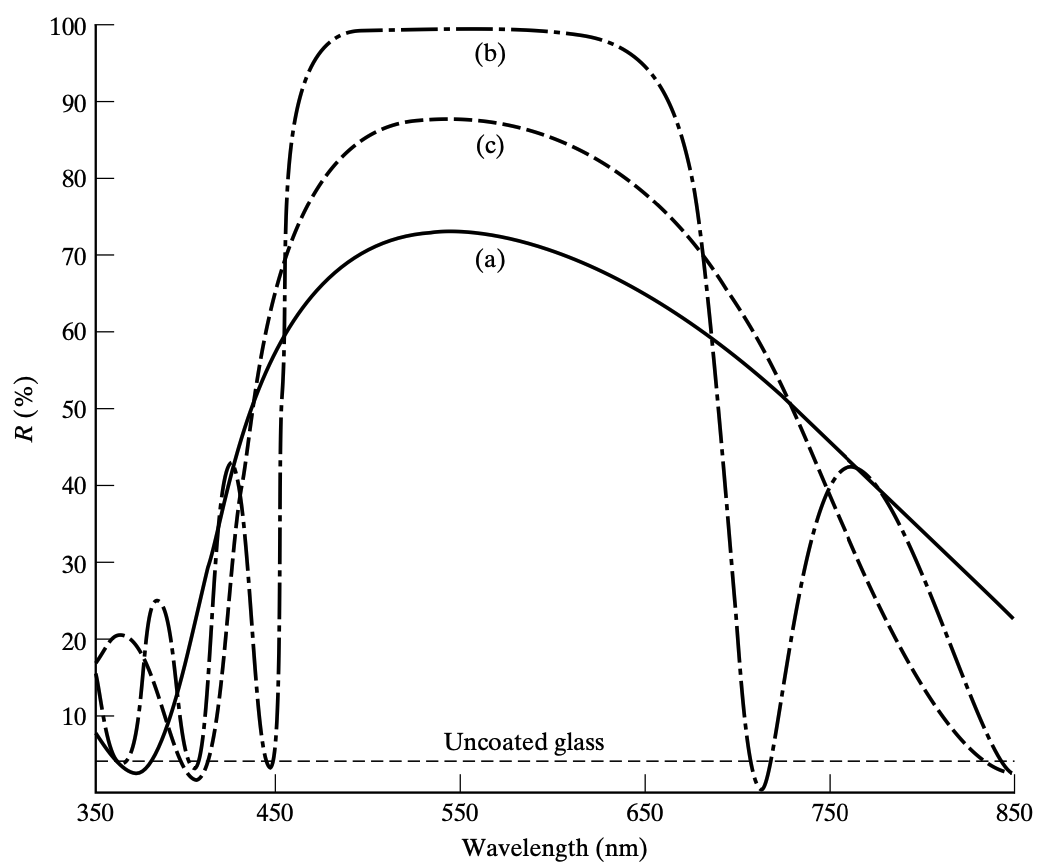
\includegraphics[width=0.4\textwidth]{Chapters/Figures/Chapter 4 Figures/High-Reflectance Graphs in the Optics Book.png}
\caption{Reflectance spectra for high-low index stacks: (a) for a two-layer double stack, (b) for a six-layer double stack, and (c) for a two-layer double stack enhanced with an additional high-index layer at the very top. Source: \cite{pedrotti_introduction_2007}}
\label{fig:Reflectance spectra from optical literature}
\end{figure}

In these configurations, layers are designed to be $\lambda/4$ thick at a design wavelength $\lambda_0 = 550$ nm. Here, the high-index material (Zinc Sulfide - ZnS) has $n_H = 2.35$, the low-index material (Magnesium Fluoride - MgF2) has $n_L = 1.38$, and the incident medium (air) has $n_0 = 1.00$. The ratio of $\frac{n_L}{n_H}$ is thus approximately $\frac{1.38}{2.35} \approx 0.587$.

Our analysis will specifically address graph (c), which demonstrates how adding an extra high-index layer between the substrate and the final low-index layer enhances maximum reflectance in a two-layer double stack ($N = 2$). This addition improves reflectance efficiency compared to simpler two-layer double configurations.

The findings showcased below stem from applying the high reflectance principles discussed in Chapter 2.

\begin{figure}[ht!]
  \centering
  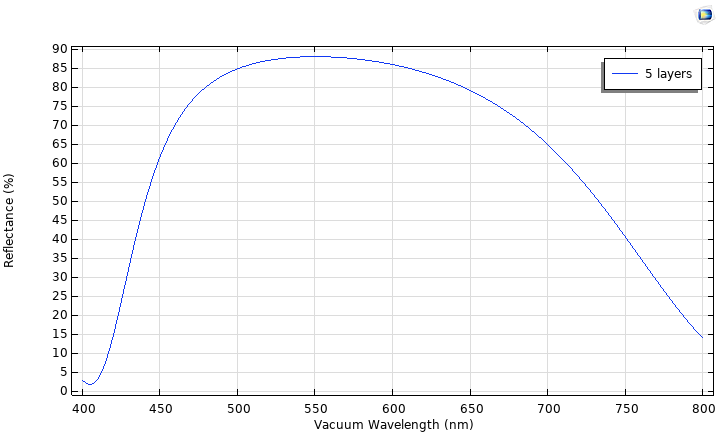
\includegraphics[width=0.4\textwidth]{Chapters/Figures/Chapter 4 Figures/High-Reflectance (5 Layers).png}
  \caption{Spectral reflectance for a structure with two pairs of high-low refractive index layers, topped with an additional high-index layer.}
  \label{fig:Reflectance 5-layer structure}
\end{figure}

Observe the alignment of peak reflectance with the textbook's findings, achieving 90%.

Employing a parametric sweep in COMSOL allows for the exploration of reflectance variation across wavelengths by systematically adjusting the count of double layer pairs ($N$) to values such as 2, 5, 10, and 20. This approach calculates solutions across a range of parameter sets. For all depicted graphs, an extra top layer with a high refractive index is incorporated to broaden the spectrum of maximum reflectance.

\begin{figure}[ht!]
  \centering
  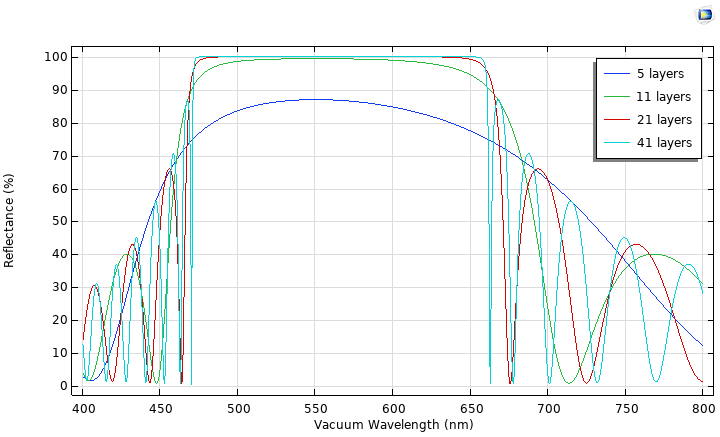
\includegraphics[width=0.4\textwidth]{Chapters/Figures/Chapter 4 Figures/High-Reflectance (5, 11, 21, and 41 Layers).png}
  \caption{Reflectance comparison for configurations with 5, 11, 21, and 41 layers, each enhanced by an additional high-index surface layer.}
  \label{fig:COMSOL multi-layer reflectance results}
\end{figure}

Unlike conventional metallic mirrors, DBRs leverage a careful and simple engineered structure of alternating thin layers of materials with contrasting refractive indices. This design typically features an odd number of layers, anchored by high refractive index materials at both ends, optimizing their reflectivity \cite{multiphysics__distributed_nodate}.

At the core of a DBR's functionality is the concept of constructive interference. As optical waves encounter the boundaries between layers, each boundary induces a partial reflection. When the optical wave's wavelength is four times the layers' optical thickness, these reflections interfere constructively, transforming the layers into an efficient reflector. This principle gives rise to a \emph{stopband}, a wavelength range where the reflector achieves heightened reflection. With an adequate number of layers, a DBR can achieve a high-quality reflection, making it useful in the operation of vertical cavity surface emitting lasers \cite{multiphysics__distributed_nodate}.

Expanding beyond the \emph{stopband}, DBRs exhibit a characteristic where reflectance transitions into a pattern of oscillating maxima and minima.

By strategically adjusting these parameters, it is possible to shift the stopband's center, enhancing the filter's spectral transmittance across a broader range. This capability to finely control the light's passage through these structures not only underscores the versatility of DBRs but also paves the way for their integration into a wide array of optical devices, where precise manipulation of light is paramount \cite{pedrotti_introduction_2007}.

Building on the principles of DBRs and their implications for enhanced reflectivity, a parallel can be drawn to PDRCS. PDRCs, which aim to achieve cooling without energy input by radiating heat into the cold outer space, can significantly benefit from the reflective properties and spectral selectivity offered by DBR structures.

PDRCs leverage similar concepts to reflect the solar spectrum while allowing the thermal infrared range to pass through effectively. By incorporating multilayer structures like those used in DBRs, PDRC devices can optimize their performance, achieving a delicate balance between high solar reflectance and high thermal emittance. This enables PDRC systems to reflect the majority of incoming solar radiation, minimizing heat absorption, while simultaneously maximizing the emission of infrared radiation for cooling.

\section{COMSOL: Modelling PDRCs}.
At Hudgings Lab, one of the simplest PDRCs has this structure. From the bottom up, silica glass serves as the base, followed by silver on top and then finally Polydimethylsiloxane (PDMS).

% TODO: INCLUDE the figure of the Glass + Silver + PDMS

% \begin{figure}[ht!]
%   \centering
%   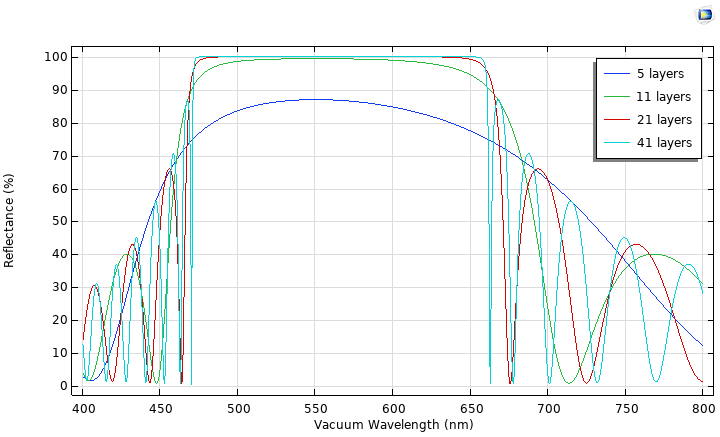
\includegraphics[width=0.4\textwidth]{Chapters/Figures/Chapter 4 Figures/High-Reflectance (5, 11, 21, and 41 Layers).png}
%   \caption{Reflectance comparison for configurations with 5, 11, 21, and 41 layers, each enhanced by an additional high-index surface layer.}
%   \label{fig:COMSOL multi-layer reflectance results}
% \end{figure}

I opted to start modelling the structure from the base up and so the results below show the results for glass, then glass plus silver, then finally glass plus silver plus PDMS where I plot the reflectance versus wavelength to see how they vary.

\subsection{Glass Layer Only.}

% TODO: INCLUDE the figure of the snippet of the COMSOL desktop setup

% \begin{figure}[ht!]
%   \centering
%   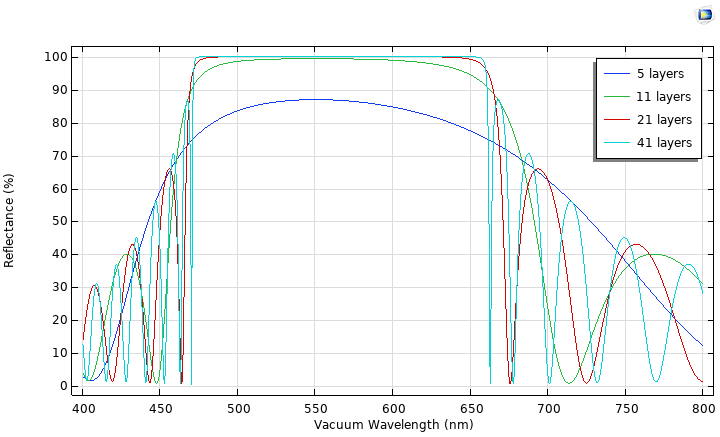
\includegraphics[width=0.4\textwidth]{Chapters/Figures/Chapter 4 Figures/High-Reflectance (5, 11, 21, and 41 Layers).png}
%   \caption{Reflectance comparison for configurations with 5, 11, 21, and 41 layers, each enhanced by an additional high-index surface layer.}
%   \label{fig:COMSOL multi-layer reflectance results}
% \end{figure}

For accurate simulations across a spectrum, it is essential to employ materials whose refractive indices are not fixed but change with wavelength. In COMSOL, this variability is addressed using an interpolation function. This function relies on a data table correlating the refractive index with specific wavelengths over a range. In COMSOL, such a function enables the simulation to adapt the material's refractive index for any given wavelength, reflecting the material's optical characteristics more realistically.

% TODO: INCLUDE figure of the snippet of the interpolation function for the Corning glass

% \begin{figure}[ht!]
%   \centering
%   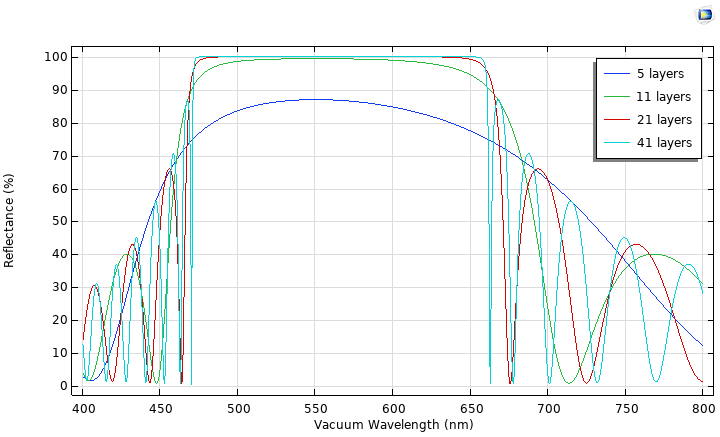
\includegraphics[width=0.4\textwidth]{Chapters/Figures/Chapter 4 Figures/High-Reflectance (5, 11, 21, and 41 Layers).png}
%   \caption{Reflectance comparison for configurations with 5, 11, 21, and 41 layers, each enhanced by an additional high-index surface layer.}
%   \label{fig:COMSOL multi-layer reflectance results}
% \end{figure}

From the interpolation table, you can plot an interpolation function to visually check how the refractive indices varies with wavelength. The function, n, allows the COMSOL model to more accurately simulate how light interacts with the material across a range of wavelengths, which is particularly important in optical simulations where dispersive effects are significant.

With this in mind, I opted to use Corning® HPFS® 7980 Fused Silica as the substrate since it came with its own interpolation function. It's important to note that one can refer to literature for experimentally determined dependence of refractive index of materials with wavelength, i.e., an interpolation function.

As expected when one plots a reflectance versus wavelength plot with just the glass (here Corning® HPFS® 7980 Fused Silica) substrate, the reflectance truly varies with wavelength.

% TODO: INCLUDE the figure of the snippet of result of JUST GLASS

% \begin{figure}[ht!]
%   \centering
%   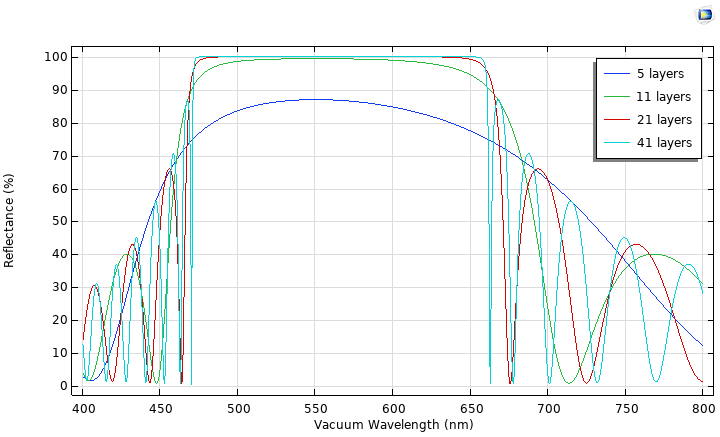
\includegraphics[width=0.4\textwidth]{Chapters/Figures/Chapter 4 Figures/High-Reflectance (5, 11, 21, and 41 Layers).png}
%   \caption{Reflectance comparison for configurations with 5, 11, 21, and 41 layers, each enhanced by an additional high-index surface layer.}
%   \label{fig:COMSOL multi-layer reflectance results}
% \end{figure}

In the range of wavelengths shown ($400 - 800$ nm), when you just have a substrate, you have a very low reflectance of less than 4\% which is not optimal if you're considering that we want to increase the reflectivity within the solar spectrum. It calls for additional materials that can satisfy the criteria for high reflectance in the solar spectrum and high emissivity in the atmospheric window. Let's deal with the former first. At Hudgings Lab, realizing that silver is a highly reflective substance, we lay it on top of the substrate to boost the potential PDRC's reflectance. Now that we've shown the results for when we just just use the glass substrate and explained the necessity of using a highly reflective substance especially in the solar spectrum, next I am going to model a glass plus silver layers.

\subsection{Glass plus Silver.}
Next, I added a silver layer on top of the glass. The need for an interpolation function for silver also persists in this case. Luckily, COMSOL has an extensive repository of silver materials with their own defined interpolation tables for their refractive indices depending on the wavelength range you would like to see your results in. For example, \emph{Ag (Silver) (Choi et al. 2020: n,k 1.23-6.99 um)} details experiments of silver's refractive indices across a range of 1.23 to 6.99 $\mu$m.

$n$ details the real part of the complex refractive index and $k$, the extension coefficient, is the imaginary part of the complex refractive index representing how much the material absorbs light.

% TODO: INCLUDE figure of the snippet of the interpolation function for Silver

% \begin{figure}[ht!]
%   \centering
%   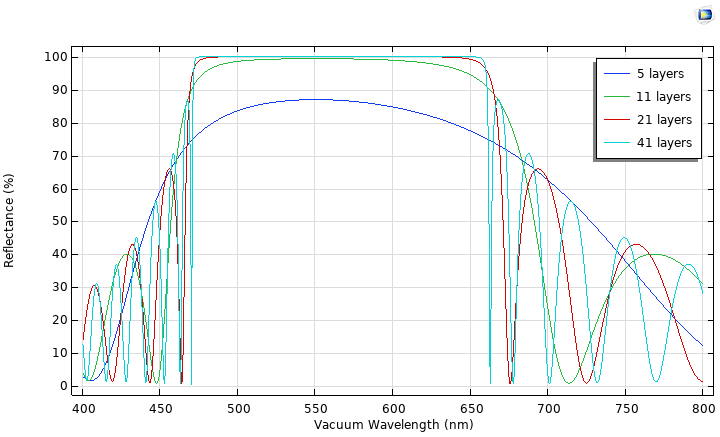
\includegraphics[width=0.4\textwidth]{Chapters/Figures/Chapter 4 Figures/High-Reflectance (5, 11, 21, and 41 Layers).png}
%   \caption{Reflectance comparison for configurations with 5, 11, 21, and 41 layers, each enhanced by an additional high-index surface layer.}
%   \label{fig:COMSOL multi-layer reflectance results}
% \end{figure}

Depending on the wavelength range one wants, there are multiple definitions of silver in the materials library of COMSOL. For instance, this silver material, \emph{Ag (Silver) (Johnson and Christy 1972: n,k 0.188-1.94 um)} details the interpolation table from 0.188-1.94 $\mu$m.

Below are the results first when I used \emph{Ag (Silver) (Johnson and Christy 1972: n,k 0.188-1.94 um)} and then when I used \emph{Ag (Silver) (Choi et al. 2020: n,k 1.23-6.99 um)}.

% TODO: INCLUDE figure glass plus silver for Johnson and Christy 1972

% \begin{figure}[ht!]
%   \centering
%   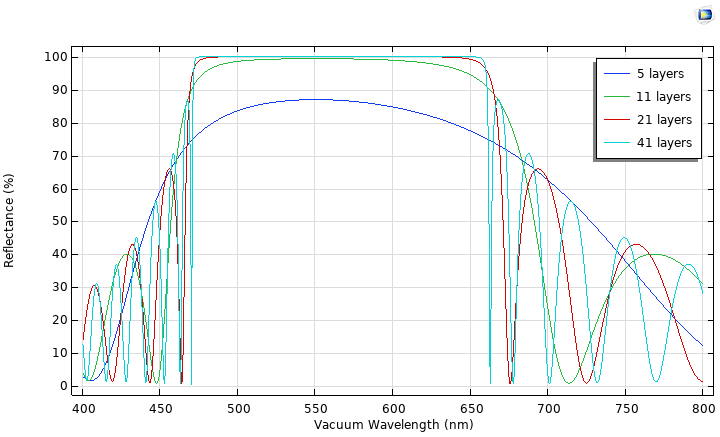
\includegraphics[width=0.4\textwidth]{Chapters/Figures/Chapter 4 Figures/High-Reflectance (5, 11, 21, and 41 Layers).png}
%   \caption{Reflectance comparison for configurations with 5, 11, 21, and 41 layers, each enhanced by an additional high-index surface layer.}
%   \label{fig:COMSOL multi-layer reflectance results}
% \end{figure}

% TODO: INCLUDE figure of glass plus silver for Choi et al. 2020

% \begin{figure}[ht!]
%   \centering
%   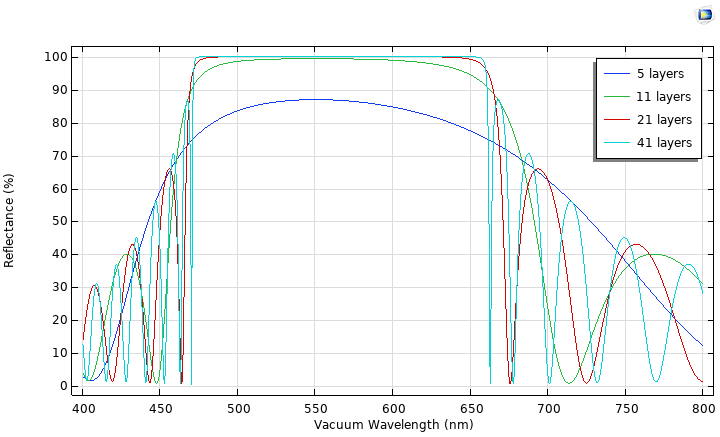
\includegraphics[width=0.4\textwidth]{Chapters/Figures/Chapter 4 Figures/High-Reflectance (5, 11, 21, and 41 Layers).png}
%   \caption{Reflectance comparison for configurations with 5, 11, 21, and 41 layers, each enhanced by an additional high-index surface layer.}
%   \label{fig:COMSOL multi-layer reflectance results}
% \end{figure}

The graphs above are a tale of mostly expected results. Indeed silver is highly reflective in the visible spectrum of wavelengths which is why we see a close to 100\% reflectance in the visible spectrum (400 - 700 nm).

\subsection{Glass plus Silver plus PDMS.}
Finally, I included a PDMS layer on top of the silver layer. Here too, I included PDMS material that already had its defined interpolation function for the refractive index. The PDMS material I used was from \emph{(C2H6OSi)n (Polydimethylsiloxane, PDMS) (Gupta et al. 2019: n 0.30-1.69 um)}.

% TODO: INCLUDE figure of glass plus silver plus PDMS results

% \begin{figure}[ht!]
%   \centering
%   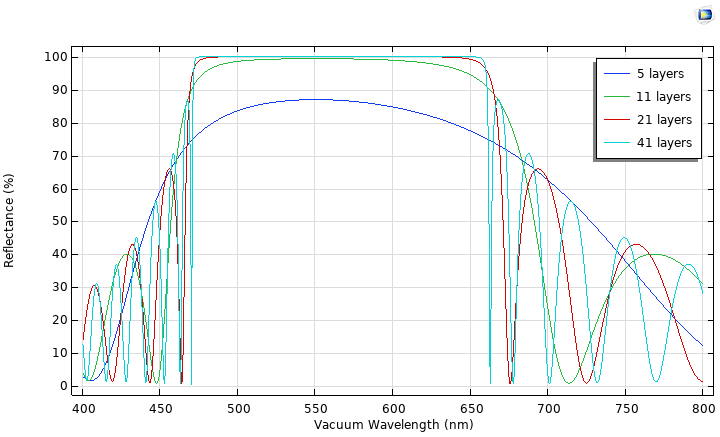
\includegraphics[width=0.4\textwidth]{Chapters/Figures/Chapter 4 Figures/High-Reflectance (5, 11, 21, and 41 Layers).png}
%   \caption{Reflectance comparison for configurations with 5, 11, 21, and 41 layers, each enhanced by an additional high-index surface layer.}
%   \label{fig:COMSOL multi-layer reflectance results}
% \end{figure}

The reflectance is also 100\% over a huge spectrum range of wavelengths.
